\documentclass[tikz,border=4pt]{standalone}
\usepackage{amsmath,amssymb}
\usepackage[compat=1.1.0]{tikz-feynman}
\usetikzlibrary{arrows.meta,positioning,automata,shapes,shapes.misc,calc,decorations.pathmorphing,decorations.markings,angles,quotes,patterns,mindmap,matrix,knots,hobby,trees}
\tikzset{->-/.style={decoration={markings, mark=at position 0.5 with {\arrow{Stealth}}}, postaction={decorate}}}
\begin{document}
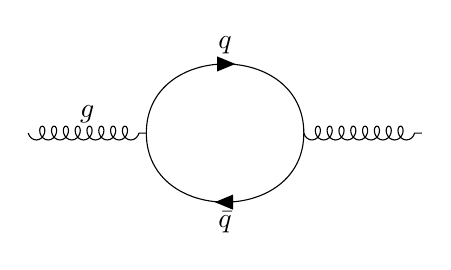
\begin{tikzpicture}
\begin{feynman}
\vertex (a); \vertex [right=1.5cm of a] (b); \vertex [right=2cm of b] (c); \vertex [right=1.5cm of c] (d);
\diagram* {
  (a) -- [gluon, edge label=\(g\)] (b),
  (b) -- [fermion, half left, edge label=\(q\)] (c),
  (c) -- [fermion, half left, edge label=\(\bar q\)] (b),
  (c) -- [gluon] (d),
};
\end{feynman}
\end{tikzpicture}
\end{document}
